%%%%%%%%%%%%%%%%%%%%%%%%%%%%%%%%%
%
%       EXERCÍCIO
%
%%%%%%%%%%%%%%%%%%%%%%%%%%%%%%%%%

\definevalorquestao

\begin{exercicioBanco}[\valorquestao]
A função afim \(f\) e a função quadrática \(g\) estão representadas a seguir.
%
\begin{center}
    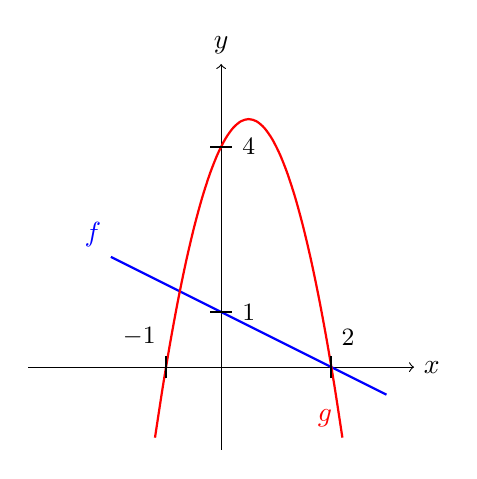
\begin{tikzpicture}[scale=0.7]
        % Eixos
        \draw[->] (-3.5,0) -- (3.5,0) node[right] {\(x\)};
        \draw[->] (0,-1.5) -- (0,5.5) node[above] {\(y\)};
              
        % Gráfico
        \draw[domain=-2:3, smooth, variable=\x, blue, thick] plot ({\x}, {-(1/2)*\x + 1});
        \node[blue, above left] at (-2, {-(1/2)*(-2) + 1}) {\(f\)};
        \draw[domain=-1.2:2.2, smooth, variable=\x, red, thick] plot ({\x}, {-2*\x*\x + 2*\x + 4}) node[above left] {\(g\)};
              
        % Pontos escolhidos
        \draw[thick] (-1,-0.2) -- (-1,0.2) node[above left]{\small\(-1\)};
        \draw[thick] (2,-0.2) -- (2,0.2) node[above right]{\small\(2\)};
        \draw[thick] (-0.2,1) -- (0.2,1) node[right]{\small\(1\)};
        \draw[thick] (-0.2,4) -- (0.2,4) node[right]{\small\(4\)};
    \end{tikzpicture}
\end{center}
%
Determine o valor de \(x < 0\) tal que \(f(x) = g(x)\).

% Define as alternativas
\newcommand{\alternativas}{%
    \begin{center}
        \begin{tabularx}{\textwidth}{XXXXX}
            (a) \(-\dfrac{3}{4}\). &
            (b) \(-\dfrac{2}{5}\). &
            (c) \(-\dfrac{4}{5}\). &
            (d) \(-\dfrac{6}{7}\). &
            (e) \(-\dfrac{2}{3}\).
        \end{tabularx}
    \end{center}
}

% Define a resposta correta
\newcommand{\resposta}{A}

% Lógica condicional para exibição
\ifdefstring{\atividade}{lista}{%
    \alternativas
    \vspace{0.5em}
    
    \noindent\textbf{Resposta:} letra \textbf{\resposta}.
}{%
    \ifdefstring{\modo}{objetivo}{%
        \alternativas
    }{%
        % modo = discursiva → não mostra alternativas
    }
}
\end{exercicioBanco}

